\documentclass[10pt,a4paper]{article}
\usepackage[utf8]{inputenc}
\usepackage[T1]{fontenc}
\usepackage{amsfonts}
\usepackage{amssymb}
\usepackage{natbib}
\usepackage{graphicx}

\title{Computer Science NEA Proposal
       \bigbreak
       \large Image Recognition from scratch}
\author{Max Cotton}
\date{}

\begin{document}

\maketitle

\section{Introduction}
\begin{figure}[h!]
\centering
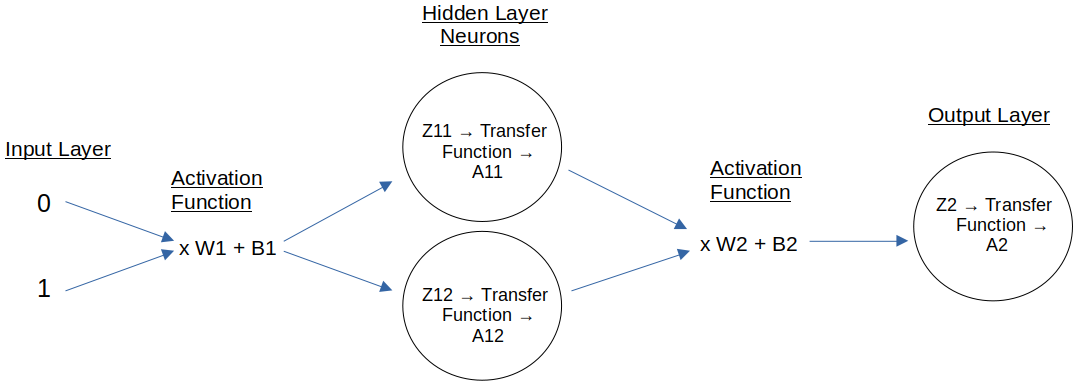
\includegraphics[width=1\textwidth]{./write-up/src/images/shallow-ann-diagram.png}
\caption{Artificial Neural Network}
\end{figure}

My project will be an investigation into how Artificial Neural Networks (ANNs) work and their applications in Image Recognition, by documenting all theory behind the 
project and developing applications of the theory, that allow for experimentation via a Graphical User Interface. 

\section{Main project objectives}

\begin{itemize}
    \item Develop and document the theory behind the project:
    \begin{itemize}
        \item To achieve this, I will derive the mathematics behind ANNs and learn the theory behind how they work. Including topics such as the following:
        \begin{itemize}
            \item Gaining a strong understanding in Matrice operations and Calculus (Such as the Chain rule, Multivariable differentiation and other laws)
            \item Learning the basic structure of ANNs, consisting of the following:
            \begin{itemize}
                \item Weights and biases
                \item Structure of layers, consisting of an input layer, hidden layer/s and an output layer
                \item The number of neurons that each layer consists of
            \end{itemize}
            \item Learning the process of Forward Propagation, where data is inputted into the feedforward ANNs to get a prediction
            \item Learning the process of Back Propagation, consisting of the following:
            \begin{itemize}
                \item The process of calculating the error/loss of the prediction, in order to show the improvement in the performance of the model as it is trained.
                \item The process of Gradient descent, in order to adjust/train the weights and biases of ANNs and learn the effects of the learing rate
                      \begin{figure}[h!]
                      \centering
                      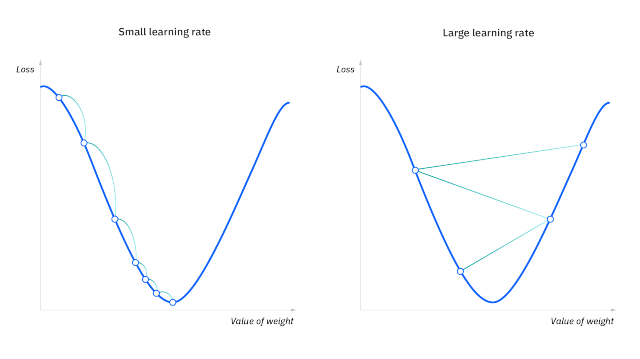
\includegraphics[width=1\textwidth]{./write-up/src/images/gradient-descent.png}
                      \caption{Gradient Descent\\
                               sourced from https://www.ibm.com/topics/gradient-descent}
                      \end{figure}
                \item The process of optimising the training, such as avoiding getting stuck in a local minima for the loss value (instead of the global) and the 
                      problem of exploding gradients (where the gradient used to update the weights and biases grows exponentially to the point of overflow errors)
            \end{itemize}
            \item Investigate the different types of ANNs, such as Perceptron and Shallow ANNs (different layer structures)
        \end{itemize}
    \end{itemize}
    \item Create ANNs:
    \begin{itemize}
        \item Create ANNs by programming them from scratch, without the use of any 3rd party Machine Learning libraries, with an object-orientated approach
    \end{itemize}
    \item Train models on datasets:
    \begin{itemize}
        \item Train the ANNs to create trained models, by learning how to provide input and output data to train the ANNs.
        \item I plan to first train an ANN model to predict the outputs of a XOR gate on two inputs of 1s and 0s, then I plan to source datasets of images from online, 
              such as the MNIST dataset (a famous dataset of images of handwritten numbers used to test the performance of ANN models), to train ANN models to predict 
              both binary and multi-class classification of images.
    \end{itemize}
    \item Create GUI to control ANNs:
    \begin{itemize}
        \item Present theory behind the project
        \item Allow for experimentation with the attributes of each ANN model (such as the learning rate and number of hidden neurons in hidden layers)
        \item Give control for training the ANNs
        \item Present the results of the trained models, such as how its prediction error/loss value changes with the number of training epochs and 
              also show its final prediction accuracy on test inputs after training.
              \begin{figure}[h!]
              \centering
              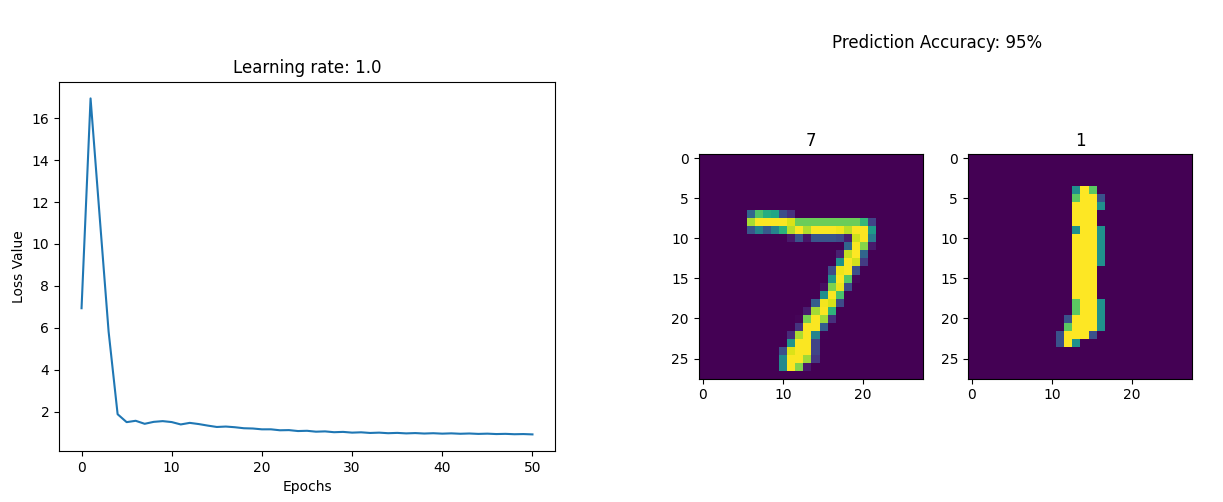
\includegraphics[width=1.2\textwidth]{./write-up/src/images/example-results.png}
              \caption{Example results of a trained model}
              \end{figure}
    \end{itemize}
    \item Experiment with expanding the project further, such as in the following ways:
    \begin{itemize}
        \item Experimenting with new ANN models, such as in the following ways:
        \begin{itemize}
            \item Effects of different Transfer Functions in training
            \item Experimenting in developing more expandable ANNs (Eg: Allowing for adding as many layers as needed and control over the number of hidden neurons in each 
                  hidden layer)
        \end{itemize}
        \item Testing improving computational power to allow for more training epochs, layers and hidden neurons (Eg: Using a GPU for calculations via Remote Access to a PC)
    \end{itemize}
\end{itemize}

\section{Programming Languages used}

\begin{itemize}
    \item I will use Python 3 for programming the ANNs and the GUI, due to its high abstraction and simple syntax to let me focus on translating the theory into code. 
          Also Python 3 has many usefull libraries for Data Science, such as NumPy for matrice manipulation and multiplication, Matplotlib for displaying data and 
          libraries for loading datasets. 
    \item I will also use Markdown, LaTex and makefile language for developing the Documentation and PDFs for the theory behind the project.        
\end{itemize}

\section{Conclusion}

I believe that learning Artificial Neural Networks and their applications in Image Recognition is a suitable focus for an Investigation project, due to the large 
quantity of content and complexity behind it and the many possible applications with it. Moreover, Artificial Intelligence is a huge field and is continuing to grow 
larger, so learning the fundamentals behind it, will help eductate the user in understanding the newest advancements in the field.

\end{document}